\documentclass[a4paper,11pt]{article}

\usepackage{amsmath,amssymb,amsfonts}
\usepackage{booktabs}
\usepackage[dvipsnames]{xcolor}
\usepackage[margin=30mm]{geometry}
\usepackage{graphicx}
	\graphicspath{
		{graphics/}
	}
\usepackage{hyperref}
	\hypersetup{
		colorlinks=true,
		linkcolor=blue,
		filecolor=blue,
		urlcolor=blue,
		citecolor=blue
	}
%\usepackage[sort&compress]{natbib}
%	\bibliographystyle{apalike}
\usepackage{soul}
\usepackage{url}


% Damien added packages
\usepackage{listings}
\lstset{language=R,
    basicstyle=\small\ttfamily,
    stringstyle=\color{DarkGreen},
    otherkeywords={0,1,2,3,4,5,6,7,8,9},
    morekeywords={TRUE,FALSE},
    deletekeywords={data,frame,length,as,character},
    keywordstyle=\color{blue},
    commentstyle=\color{DarkGreen},
}
\usepackage{float}
\usepackage{subfig}

\newcommand{\jwj}[1]{{\color{red}{~(jwj: #1)}}}
\newcommand{\yourInitials}[1]{{\color{blue}{~(yourInitials: #1)}}}

\usepackage{titlesec}
\titleformat{\section}{\normalfont\large\bfseries}{}{0pt}{}
\titleformat{\subsection}{\normalfont\large\bfseries}{}{10pt}{}
\titleformat{\subsubsection}{\normalfont\small\bfseries}{}{30pt}{}


%=======================================

%Note: Include constraints that ensure if i=1 is selected, all t's in i=1 must be activated too. If i is on then all t's must be on too.

\title{BOZ780 Assignment 3}
\author{DS de Gouveia \\ 15003079}
\date{\today}

\begin{document}
\maketitle
\tableofcontents
\newpage

%=======================================================================
\section{Question 1 - Farmer Jones}

The following assumptions are made. At the start of each week Farmer jones decides how much feed $p$ to allot to his steer. At the start of the 11th week farmer Jones may ONLY sell the steer for R25/kg and cannot feed the steer in the final week. He cannot sell the steer in the weeks leading to its sale either.

The recursion function $f_t(w_t, p_t)$ can be defined as

\vspace{12pt}

\begin{tabular}{p{0.12\linewidth}  p{0.78\linewidth}}
	$f_t(w_t,p_t) \triangleq$ & the maximum profit (Rands) for the steer during stages $t,t+1,\dots, T$ given that the steer is allotted $p_t$ kilograms of feed and weighs $w_t$ kilograms at the start of stage $t$. \\
	$c(p_t)\triangleq$ & the cost (Rands) to feed the steer $p_t$ kilograms of feed at each stage $t$. \\
	$g(w_t, p_t) \triangleq$ & the mass of the steer (kilograms) at the end of stage $t$, given its mass $w_t$ (kilograms) and the feed $p_t$ (kilograms) allotted to it at the start of stage $t$.
\end{tabular}
 
 \vspace{12pt}
 
 During the final week, no feed is allotted to the steer and thus, no growth takes place. For the last stage $t=T=10$ the recursion function can be defined as

\begin{equation}
	f_{11}(w_{11},p_{11}) = \max \{25w_{11}	\}
\end{equation}

which ensures that starting mass $w_{11}$ of week $T$ is as large as possible to maximise profitability. During the preceding weeks, the steer was fed, grew and accrued a cost. The profitability of preceding weeks is determined by the end mass at sale. Thus, the recursion function for $t<T$ can be defined as

\begin{equation}
	f_t(w_t,p_t) = \max \{f_t(g(w_t,p_t),p_t)- c(p_t)	\}
\end{equation}

where $g(w_t,p_t)$ is the mass of the steer at the end of week 10 (start of week 11) given the starting mass $w_t$ and allotted feed $p_t$. 

The starting mass of week 11 is equal to the end mass of week 10 given the allotted feed, $m_{11} =g (w_{10},p_{10})$. As the final mass is converted into a Rand value, the allotted feed $p_t$, is converted into an accrued cost, $c(p_t)$. Both the amount at sale and cost for each week is carried from week 11 to week 1. This enables farmer Jones to evaluate the many trade offs with feeding the steer during each week.

It should be noted that the mass of the animal is not evaluated within the recursion function however the mass must still be captured. The mass of the steer at any point in time can be evaluated as

\begin{align}
	w_t = \sum_{t=2}^Tg(w_{t-1},p_{t-1}) & &t\in \{2,\dots,11\}
\end{align}

where $w_t$ is an accumulative function, dependent on the previous mass and feed requirement. The initial mass $w_1, t=1$ is a starting parameter. The feed allotted to an animal, $p_t$ has been parametrised to keep track of the feed issued at each stage, however, it can be simplified to merely $p$, the feed allotted at each stage.

\newpage

%=======================================================================
\section{Question 2 - Number of crimes}

Each precinct has rate of improvement, defined as the current crime given number of patrol cars less future crime with an additional patrol car. The highest reduction in crime is seen as the better solution. For five planning stages, a single additional patrol car is assigned to the precinct with the greatest improvement. This process continues until the termination of the planning stages which implies that a maximum of five cars have been allocated. This recursive approach is viable as each proceeding improvement increases from its
 predecessor.

\vspace{12pt}

\begin{tabular}{p{0.1\linewidth}  p{0.8\linewidth}}
$n_{i} \triangleq$ & number of patrol cars assigned to precinct $i$, where $i = \{1,2,3\}$  \\ 
  $f_s(n_{i}) \triangleq$&  maximum crime reduction rate for precinct $i$ in planning state $s$ for $s,s+1,\dots, 5$ given $n_i$ number of patrol cars\\
    $c_i(n_i) \triangleq$ & crime reduction rate for precinct $i$ during planning stage $s$ given $n_i$ number of patrol cars
\end{tabular}

\vspace{12pt}

The inclusion of $c_i(n_i)$ simplifies the problem, reducing the complexity of the recursion function, which can be modelled as 

\begin{align}
	f_s(n_i) &= \max_{\sum_{i=1}^5 n_i\leq 5} \{c_i(n_i)\}
\end{align}

where $f_s(n_i)$ attempts to identify the maximum reduction in crime rates for each  additional patrol car $n_i$ is added to precinct $i$. The values for $c_i(n_i)$ are available in Table~\ref{Q2:Tbl1}. During each planning phase, a single patrol car is added and the precinct with the greatest improvement is then selected. The number of patrol cars for each precinct are store in memory and used in the next stage.

\begin{table}[h]
\centering
\caption{Difference in crime rates per number of patrol cars.}
\begin{tabular}{c|ccc}
\hline
\textbf{n} & \textbf{Precinct 1} & \textbf{Precinct 2} & \textbf{Precinct 3} \\ 
&$i=1$ &$i=2$ &$i=3$  \\
\hline
1&	4&	6&	6 \\
2&	3&	3&	3\\
3&	3&	2&	3\\
4&	3&	2&	2\\
5&	1&	1&	1\\
\hline
\end{tabular}
\label{Q2:Tbl1}
\end{table}


\begin{align}
	f_1(1) &= \max 
	\begin{Bmatrix}
		\text{Precint 1}: & c_1(1) = 4 \\
		\text{Precint 2}: & c_2(1) =6 \\
		\textbf{Precint 3}: & c_3(1) =6
	\end{Bmatrix}	
\end{align}
\begin{align}
	f_2(2) &= \max 
	\begin{Bmatrix}
		\text{Precint 1}: & c_1(1) = 4 \\
		\textbf{Precint 2}: & c_2(1) =6 \\
		\text{Precint 3}: & c_3(2) =3
	\end{Bmatrix}	
\end{align}
\begin{align}
	f_3(3) &= \max 
	\begin{Bmatrix}
		\textbf{Precint 1}: & c_1(1) = 4 \\
		\text{Precint 2}: & c_2(2) =3 \\
		\text{Precint 3}: & c_3(2) =3
	\end{Bmatrix}	
\end{align}
\begin{align}
	f_4(4) &= \max 
	\begin{Bmatrix}
		\textbf{Precint 1}: & c_1(2) = 3 \\
		\text{Precint 2}: & c_2(2) =3 \\
		\text{Precint 3}: & c_3(2) =3
	\end{Bmatrix}	
\end{align}
\begin{align}
	f_5(5) &= \max 
	\begin{Bmatrix}
		\textbf{Precint 1}: & c_1(3) = 4 \\
		\text{Precint 2}: & c_2(2) =6 \\
		\text{Precint 3}: & c_3(2) =6
	\end{Bmatrix}	
\end{align}

The resulting allocation yields 37 cases of reported crime across the three precincts, with the allocation to each precinct summarised in Table~\ref{Q2:Tbl1}.

\begin{table}[h]
	\centering
	\caption{Final solution allocates three cars to the first precinct, and a single car to both the second and third precinct.}
	\label{q2:finalSol}
	\begin{tabular}{c|ccc}
	\hline
		& \textbf{Patrol cars} & \textbf{Crime} \\
		\hline
		\text{Precinct 1} &3 & 4\\
		\text{Precinct 2} &1 & 19\\
		\text{Precinct 3} &1 & 14\\
		\hline
		\textbf{Total} & 5 & 37\\
		\hline
	\end{tabular}
\end{table}


The prescribed solution is, however, not the only viable and optimal solution. Alternative solutions become possible after the third planning phase, that is, once all precincts have been allocated a single car. Figure~\ref{q2fig:many} describes that a maximum of two cars be be assigned to precinct 1 or 3 after the third planning stage. At most, precinct 2 can have two cars assigned to it. 

\begin{figure}[h]
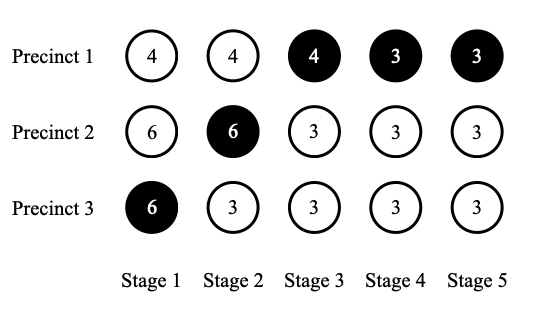
\includegraphics[width=9cm]{q2Solution.png}
\centering
\caption{Graphical approach based on the selecting the precinct that would benefit most from an additional patrol car.}
\end{figure}





\begin{figure}[h]
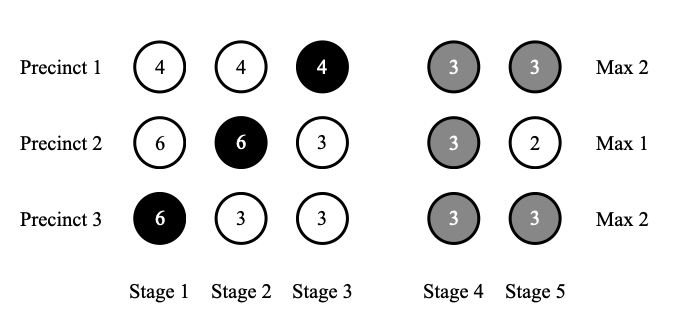
\includegraphics[width=11cm]{q2Many.png}
\centering
\caption{Several possible, optimal solutions exist within stage 4 and 5. The upper limits of each are noted to right of the figure.}
\label{q2fig:many}
\end{figure}


\newpage
%=======================================================================
\section{Question 3 - Maintenance regime}

It is assumed that when maintenance is conducted on the machine, no downtime is occurs and the machine can generate revenue during the same week maintenance is conducted.

The recursion function $f_t(x_t)$ is defined as
\vspace{12pt}

\begin{tabular}{p{0.1\linewidth}  p{0.8\linewidth}}
	$f_t(x_t) \triangleq$ & maximum net profit (Dollars) generated by the machine in stage (week) $t,t+1,\dots, T$ given the state $x_i$ \\ 
  	$x_t \triangleq$&  binary variable denoting the state of the machine at stage $t$ where $i =\{1,0\}$ with 1 = Running, 0 = Broken \\
\end{tabular}

\vspace{12pt}

If the machine is running we are certain of making \$100. We must then determine if the additional cost of maintenance will bring us additional revenue in future states. Starting from the final state and working backwards, two possible outcomes (running, broken) and four possible actions (none, maintain, repair, replace) are available. The chosen action impacts the profitability of the operation. 

\begin{table}[h]
	\centering
	\label{q3:revCalc}
	\begin{tabular}{ccccc}
	\hline
		\textbf{Action $i$} & \textbf{Revenue(\$)} & \textbf{Cost(\$)}& \textbf{Profit(\$)}\\
		\hline
		\text{None} &100 & 0 &100\\
		\text{Maintenance} &100 & 20&80\\
		\text{Repair} &100 & 40& 60\\
		\text{Replace} &100 & 90&10\\
		\hline
	\end{tabular}
\end{table}

The profit in the final stage is dependent on preceding actions thus, the possible profit earned in state 4 depends on the action and associated likelihood of the action in stage 3. Essentially, all future profits are at risk when selecting an action, however the proceeding outcome of running is always desired. This way, we evaluate the future decision with the assumption that the machine will be running as illustrated in Figure~\ref{q3:Fig}. The recursion function for the last stage $t=T=4$ must be defined for $x_t=1$ and $x_t=0$ as neither states are known with certainty.

\begin{equation}
	f_4(1)= \max \begin{Bmatrix}
		\text{None} & 100*0.3 = 30 \\
		\text{Maintenance}& 80 *0.6 = 48 
	\end{Bmatrix}
\end{equation}

\begin{equation}
	f_4(0)= \max \begin{Bmatrix}
		\text{Repair}& 60*0.4 = 24 \\
		\text{Replace}& 10*1 =  10
	\end{Bmatrix}
\end{equation}

For $1<t<T$ the recursion function can be defined as follows.

\begin{equation}
	f_t(1)= \max \begin{Bmatrix}
		\text{None} & 0.7f_{t+1}(0)+0.3f_{t+1}(1)  \\
		\text{Maintenance}& 0.4f_{t+1}(0)+0.6f_{t+1}(1) 
	\end{Bmatrix}
\end{equation}

\begin{equation}
	f_t(0)= \max \begin{Bmatrix}
		\text{Repair}& 0.4f_{t+1}(0)+0.6f_{t+1}(1)  \\
		\text{Replace}& 0+1.0f_{t+1}(1) 
	\end{Bmatrix}
\end{equation}

The decision to be made during stage $t$ given state $x_t$ is evaluate against possibly obtaining the revenue in the future state $t+1$. Lastly, as we know that during the first week the machine was running, the recursion function for $t=1$ can be defined as follows.

\begin{equation}
	f_1(1)= \max \begin{Bmatrix}
		\text{None} & 0.7f_{t+1}(0)+0.3f_{t+1}(1)  \\
		\text{Maintenance}& 0.4f_{t+1}(0)+0.6f_{t+1}(1) 
	\end{Bmatrix}
\end{equation}

The final stage $t=4$ is evaluated first moving towards the initial stage $t=1$. During each stage, the action which yields the largest profit is chosen and noted, until all stages are evaluated. The outcome is a confirmed maintenance schedule that is estimated to maximise profitability.

\begin{figure}[h]
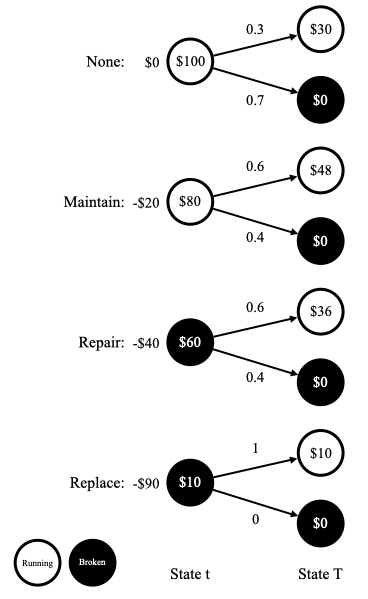
\includegraphics[width=7cm, height=11cm]{q3States.png}
\centering
\caption{The final state $T$ is dependant on preceding states and to account for the uncertainty we multiply the revenue (less costs) by the likelihood of achieving that revenue given the state and action.}
\label{q3:Fig}
\end{figure}



\newpage
%=======================================================================
\section{Question 4 - Investments}
The objective of this problem is to allocate an amount of money into one of three projects that will yield the greatest probable return. The probable return for each project $i$, given an amount of investment capital $n_i$ in dollars, is calculated as the Net Present Value (NPV) multiplied by the probability of the investment achieving its NPV. The probable return's of each investment associated with each project $i$ for a given investment amount $n_i$ are then summated. The difference between the summated probable return for each $n_i$ amount are then calculated. With reference to Table~\ref{q4:tblCis} a cost function $c_i(n_i)$ can be derived to determine the improvement by increasing $n_i$ for each project such that
\begin{align}
	c_1(1) &= 2.9 \\
	c_1(2) &= 2 \\
	c_1(3) &= 2 \\
	c_1(4) &= 2.1
\end{align}

with the remaining values present in Table~\ref{q4:tblCis}. Abstracting the problem in form, in my opinion, simplifies the solution approach. A simple recursion may then be defined as

\vspace{12pt}

\begin{tabular}{p{0.1\linewidth}  p{0.8\linewidth}}
	$f_s(n_i) \triangleq$ & maximum investment return (million dollars) in planning stage $s, s+1,\dots,S$ for project $i$ given capital investment $n_i$ \\
	$c_i(n_i) \triangleq$ & investment improvement (million dollars) for project $i$ given $n_i$
\end{tabular}

\vspace{12pt}

The recursion function $f_i(n_i)$ is implemented as
\begin{equation}
	f_i(n_i) = \max_{n_i}\{c_i(n_i)\}
\end{equation}

As this problem has been abstracted in such a form, we move from the simple decision to the complex one that is $s = 1$ to $s = S = 4$.
\begin{align}
	f_1(1) &= \max 
	\begin{Bmatrix}
		\text{Project 1}: & c_1(1) = 2.9 \\
		\text{Project 2}: & c_2(1) =1.7 \\
		\textbf{Project 3}: & c_3(1) =3.4
	\end{Bmatrix}
\end{align}	

\begin{align}
	f_2(2) &= \max 
	\begin{Bmatrix}
		\textbf{Project 1}: & c_1(1) = 2.9 \\
		\text{Project 2}: & c_2(1) =1.7 \\
		\text{Project 3}: & c_3(2) =2
	\end{Bmatrix}
\end{align}	
At this point there are two possible choices that may be made.Option 1, select project 1 and option 2 select project 3 and then project 1. Option 1 proceeds as follows.
\begin{align}
	f_3(3) &= \max 
	\begin{Bmatrix}
		\textbf{Project 1}: & c_1(2) = 2 \\
		\text{Project 2}: & c_2(1) =1.7 \\
		\text{Project 3}: & c_3(2) =2
	\end{Bmatrix}
\end{align}	

\begin{align}
	f_4(4) &= \max 
	\begin{Bmatrix}
		\textbf{Project 1}: & c_1(2) = 2 \\
		\text{Project 2}: & c_2(1) =1.7 \\
		\text{Project 3}: & c_3(2) =2
	\end{Bmatrix}
\end{align}	

Option 2 proceeds as follows.
\begin{align}
	f_3(3) &= \max 
	\begin{Bmatrix}
		\text{Project 1}: & c_1(2) = 2 \\
		\text{Project 2}: & c_2(1) =1.7 \\
		\textbf{Project 3}: & c_3(2) =2
	\end{Bmatrix}
\end{align}	

\begin{align}
	f_4(4) &= \max 
	\begin{Bmatrix}
		\textbf{Project 1}: & c_1(2) = 2 \\
		\text{Project 2}: & c_2(1) =1.7 \\
		\text{Project 3}: & c_3(2) =1.3
	\end{Bmatrix}
\end{align}	

There are other variations in the manner of assignment however there are only two optimal possibilities. The first is to assign \$3 million to project 1 and \$1 million to project 3. The second is to assigned \$2 million to both project 1 and 2. Both options result in a total NPV of \$10.3 million dollars. 

This approach work as the future value depends on the previous value. Instead of including this dependency within the recursion function it is evaluated beforehand to both simplify the model and reduce computational complexity.

\begin{table}[]
\centering
\begin{tabular}{ccccc|c|c}
\hline
\textbf{Project} & \textbf{Dollars} & $NPV_1*P_1$ & $NPV_2*P_2$ & $NPV_3*P_3$ & \textbf{Sum} & \textbf{Difference} \\

\hline
1                & 1                & 1,2                 & 1,2                 & 0,5                 & 2,9          & 2,9           \\
                & 2                & 1,5                 & 1,8                 & 1,6                 & 4,9          & 2             \\
                & 3                & 2,4                 & 3,5                 & 1                   & 6,9          & 2             \\
                & 4                & 1,4                 & 3,6                 & 4                   & 9            & 2,1           \\ \hline
2                & 1                & 0,5                 & 0,8                 & 0,4                 & 1,7          & 1,7           \\
                & 2                & 1,2                 & 2                   & 1,2                 & 4,4          & 2,7           \\
                & 3                & 1,2                 & 1,8                 & 3,2                 & 6,2          & 1,8           \\
                & 4                & 1,2                 & 2,4                 & 2,7                 & 6,3          & 0,1           \\ \hline
3                & 1                & 0                   & 2,4                 & 1                   & 3,4          & 3,4           \\ 
                & 2                & 1,6                 & 2,4                 & 1,4                 & 5,4          & 2             \\
                & 3                & 1,5                 & 2,8                 & 2,4                 & 6,7          & 1,3           \\
                & 4                & 0,6                 & 4                   & 3,6                 & 8,2          & 1,5          \\
\hline
\end{tabular}
\caption{Probable investment outcomes for each each project given an amount to invest in}
\label{q4:tblCis}
\end{table}

\end{document}
